\documentclass[a4paper, 11pt]{article}
\usepackage{theme}
\usepackage{shortcuts}
\addbibresource{ref.bib}

\title{Starting project report} % : Semantic Classification of 3D point clouds with multiscale spherical neighborhoods}
\author[1, 2]{Ines VATI}
% \affil[1]{École des Ponts ParisTech, Champs-sur-Marne, France}
% \affil[2]{MVA, ENS Paris-Saclay, Cachan, France}
% \affil[1, 2]{Email \email{ines.vati@eleves.enpc.fr}}


\date{}

\begin{document}
\maketitle
% \begin{abstract}
    
% \end{abstract}
% \textbf{Keywords. } 3D point clouds, semantic classification, multiscale, spherical neighborhoods, Random Forest

\section{Article summary}
The goal of the studied article \cite{thomas_semantic_2018} is to classify each point of a 3D point clouds using an innovative approach to design features which will be employ by a random forest classifier. 
% The features are computed using a new definition of multiscale neighborhoods using spherical neighborhoods and proportional subsampling. 
% Classical definition of local point neighborhoods are spherical, k-nearest neighbors (KNN) neighborhoods, and also cylindrical neighborhoods. The inconvenience of these approaches is that it requires to determine the scale of the neighborhood.

\textbf{Main contributions. } The authors leverage a multiscale approach that has been proven to be more accurate. Their features computing with multiscale spherical neighborhoods are more effective than state of the art features and scales well to large scale datasets. 
% Their method keeps the features undistorted while ensuring sufficient density at each scale.

\section{First Implementation results}
My code is available on \url{https://github.com/InesVATI/npm3d-project}.

I want to implement the method from scrath as no code were available. I will apply their method on the Paris-rue-Cassette dataset\footnote{\url{http://data.ign.fr/benchmarks/UrbanAnalysis/}} (12 millions points). The ground truth raw contained a large number of classes. I had to parse an XML file to group together some label classes to fairly compare the results with those obtained in the articles. For this dataset, the number of points for each classes is given in the table \ref{tab:classes}. The classes are higly unbalanced.

\textbf{Multiscale features computation.} Let consider $N$ points of interest for which we want to compute the multiscale features. The features are given in the table \ref{tab:thomas_feat}. $S$ is the number of scales. The features are computed using the following steps:

\begin{enumerate}
    \item At scale 0, I compute the eigenvalues and eigenvectors of the covariance matrix of the neighborhood with a radius $r_0$ and I compute the 18 features for each point of interest at this scale
    \item  For each scale $s$, I apply a grid subsampling on the original cloud with a voxel size $r/\rho$. Each original point is assigned to the closest voxel center and will have the same features as the voxel center. 
    \item I compute the 18 features for each voxel center associated with at least one point of interest at this scale, on a spherical neighborhood of radius $r_s = r_0 * \rho^s$
    \item I then obtain a feature matrix of size $N \times 18 * S$.
\end{enumerate}

For now, the feature computation is quite long. I applied the classification on the MiniLille (1,901,853 and 2,500,428 points) and MiniParis (4,159,318 points) datasets from \href{https://npm3d.fr/benchmark-for-master-course-on-3d-point-clouds}{NPM3D benchmark}. This dataset is small but it allows me to evaluatue how the method generalizes to unseen data. It took 370s to compute the features of 9,600 points. 

I thought about computing the feature of all points in the Paris-rue-Cassette dataset and save the result but it take too much time. I am thinking about using JAX for improve the computation time but I am not sure that it will be enough.

% \bfseries{Random Forest classifier.}


\section{Perspectives}
The things that I plan to do are :
\begin{itemize}
    \item improving computation time using JAX ?
    \item plotting histograms of the neighborhood sizess for different scales to check they are not too small
    \item comparing the proposed method with a state of the art method on a small dataset (MiniLille or MiniParis) like the one proposed by \cite{hackel_fast_nodate} or on a more recent method 
\end{itemize} 

\textbf{Improvement proposals.} For the project, we also have to propose improvements. I will propose to  add height features as suggested by Hackel et al. \cite{hackel_fast_nodate}. They are said to better describe the vertical and/or thin objects like traffic signs or tree trunks. I am also thinking of using another classifier different from a random forest like a Multilayer Perceptron algorithm. 

\printbibliography

\appendix 
\section{Label points distribution in the Paris-rue-Cassette dataset}
\begin{table}[H]
    \centering
    \begin{tabular}{|c|c|c|}
        Class name & Label & Number of points \\
        Ground & 1 & 4229639\\ 
        Building & 2 & 7027016 \\ 
        Traffic Signs & 3 & 1355\\ 
        Pedestrian & 4 & 23999\\ 
        Cars & 5 & 368271\\ 
        Vegetation & 6 & 212131\\ 
        Motorcycles & 7 & 38330\\ 
    \end{tabular}
    \caption{Number of points for each class for the Paris-rue-Cassette dataset. The label 0 is for the remaining unclassified points.}
    \label{tab:classes}
\end{table}
\begin{figure}[H]
    \centering
    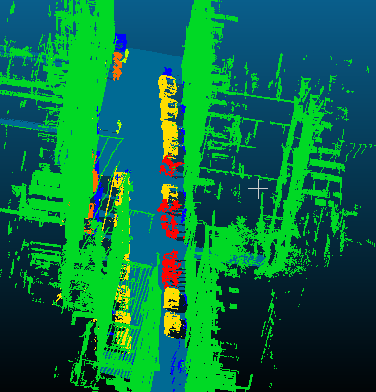
\includegraphics[width=\textwidth]{../Figures/GT_forClassification.png}
    \caption{Ground truth for the Paris-rue-Cassette dataset with the 7 classes.}
\end{figure}

\section{Multiscale features computation}
\begin{table}[H]
    \centering
    \begin{tabular}{|c||c|}
    \hline   
    Sum of eigenvalues & $\sum \lambda_i$ \\[1ex]
    \hline
    Omnivariance & $(\prod \lambda_i)^{(1/3)}$\\[1ex]
    \hline
    Eigenentropy & $-\sum \lambda_i \ln(\lambda_i)$\\[1ex]
    \hline
    Linearity & $\frac{\lambda_1 - \lambda_2}{\lambda_1}$\\[1ex]
    \hline
    Planarity & $\frac{\lambda_2 - \lambda_3}{\lambda_1}$\\[1ex]
    \hline
    Sphericity & $\frac{\lambda_3}{\lambda_1}$\\[1ex]
    \hline
    Change of curvature & $\lambda_1 - \lambda_3$\\[1ex]
    \hline
    Verticality ($\times2$) & $|\arcsin(\dotp{e_i}{e_z})|_{i=1, 3}$ \\[1ex]
    \hline
    Absolute moment ($\times6$) & $\frac{1}{|\mathcal{N}|}|\sum_{j\in\mathcal{N}} \dotp{p_j - \mathbf{p}}{e_i}^k|_{k = 1, 2;\; i = 1, 2, 3}$\\[1ex]
    \hline  
    Vertical moment ($\times2$) & $\frac{1}{|\mathcal{N}|}|\sum_{j\in\mathcal{N}} \dotp{p_j - \mathbf{p}}{e_z}^k|_{k=1, 2}$ \\[1ex]
    \hline
    Number of points & $|\mathcal{N}|$\\[1ex]
    \hline
    \end{tabular}
    \caption{Geometric features \cite{thomas_semantic_2018} of point $\mathbf{p}$ whose neighborhood is $\mathcal{N}$.}
    \label{tab:thomas_feat}
\end{table}
\end{document}